%=======================================================
% CHAPTER 1: LATTICES
%=======================================================

\begin{frame}[plain]
  \begin{center}\bfseries\centering
    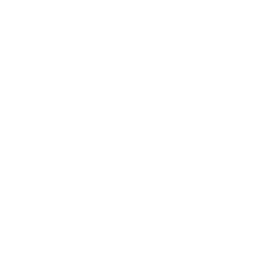
\includegraphics[scale=1]{assets/branding/opa0}
    \vspace{-5.75cm}\\
    {\adjustbox{scale=2.15}{\color{TealDarkCyan}\;II.\;Lattices}}
    \vspace{.25cm}
    \begin{minipage}{.78\textwidth}
      \scriptsize\color{Ink}
      \textbf{Big picture.}\; A basis is a coordinate description; the lattice is the invariant geometric object.\\[.2cm]
      \textbf{Details to watch.}\; integer combinations, basis changes, covolume, dual lattices, and Gram matrices.
    \end{minipage}
    {\ }\vspace{2.1cm}\\
    \bigskip
  \end{center}
\end{frame}

\begin{frame}[shrink=6]{\textbf{II. Lattices}}{Definition}
\defbox[Lattice generated by a basis]{
Let $b_1,\ldots,b_n\in\R^m$ be linearly independent. The lattice generated by them is
\[
  \Lat(\mat B)=\set{\sum_{i=1}^n z_i b_i : z_i\in\Z}
  = \mat B\Z^n,
\]
where $\mat B=[b_1\ \cdots\ b_n]\in\R^{m\times n}$.
}
\begin{itemize}
  \item The rank is $n$.
  \item The ambient dimension is $m$.
  \item A full-rank lattice in $\R^n$ has $m=n$.
\end{itemize}
\textbf{Equivalent viewpoint.}\; A lattice is a discrete additive subgroup of $\R^m$.

\textbf{Concrete example.}\; With $b_1=(2,0)$ and $b_2=(1,3)$,
\[
  \Lat=\set{u(2,0)+v(1,3):u,v\in\Z}
  =\set{(2u+v,3v):u,v\in\Z}.
\]
Thus $(4,6)=1b_1+2b_2\in\Lat$, while $(1,0)\notin\Lat$.
\end{frame}

\begin{frame}{\textbf{II. Lattices}}{Visualization: Integer Coordinates Become Geometry}
\small
\begin{center}
\begin{tikzpicture}[scale=.72]
  \begin{scope}[shift={(-4.1,-.55)}]
    \foreach \i in {-2,...,2}{
      \draw[thin lattice line] (\i,-2.2) -- (\i,2.2);
      \draw[thin lattice line] (-2.2,\i) -- (2.2,\i);
    }
    \foreach \i in {-2,...,2}{
      \foreach \j in {-2,...,2}{
        \node[lattice point] at (\i,\j) {};
      }
    }
    \draw[basis vector] (0,0) -- (1,0) node[below] {$e_1$};
    \draw[basis vector] (0,0) -- (0,1) node[left] {$e_2$};
    \node[circle,fill=ErrorRed,inner sep=2pt,label={[tiny label]above:$(2,1)$}] at (2,1) {};
    \node[caption text] at (0,-2.65) {coefficient lattice $\Z^2$};
  \end{scope}

  \node[process blue,align=center] (map) at (0,0.65)
    {$\mat B=\begin{bmatrix}2&1\\0&3\end{bmatrix}$\\[2pt]multiply by $\mat B$};
  \draw[flow blue] (-1.55,.55) -- (map.west);
  \draw[flow blue] (map.east) -- (1.55,.55);

  \begin{scope}[shift={(3.55,-.95)},scale=.46]
    \foreach \i in {-2,...,2}{
      \foreach \j in {-2,...,2}{
        \node[lattice point] at ({2*\i+\j},{3*\j}) {};
      }
    }
    \draw[basis vector] (0,0) -- (2,0) node[below] {$b_1=(2,0)$};
    \draw[basis vector] (0,0) -- (1,3) node[right] {$b_2=(1,3)$};
    \draw[short vector] (0,0) -- (5,3) node[above right] {$2b_1+b_2=(5,3)$};
    \node[circle,fill=ErrorRed,inner sep=2.5pt] at (5,3) {};
    \node[caption text,scale=1.15] at (1,-4.7) {$\mat B\Z^2$};
  \end{scope}
\end{tikzpicture}
\end{center}
\[
  (u,v)\in\Z^2\quad\longmapsto\quad u b_1+v b_2=(2u+v,3v).
\]
\textbf{Point.}\; A lattice basis is a linear machine that turns integer coordinates into a discrete geometric point set.
\end{frame}

\begin{frame}[shrink=8]{\textbf{II. Lattices}}{Many Bases, One Lattice}
\begin{columns}[T,onlytextwidth]
\begin{column}{.54\textwidth}
\thmbox[Change of basis]{
If $\mat B$ is a basis matrix and $\mat U\in\GL_n(\Z)$ is unimodular, then
\[
  \Lat(\mat B\mat U)=\Lat(\mat B).
\]
Conversely, two full-rank bases of the same lattice differ by such a matrix.
}
\begin{itemize}
  \item Unimodular means $\mat U$ has integer entries and determinant $\pm 1$.
  \item The lattice is the invariant object; the basis is only a coordinate choice.
\end{itemize}
\textbf{Example.}\; For $\mat U=\begin{bmatrix}1&1\\0&1\end{bmatrix}$,
\[
  [b_1\ b_2]\mat U=[b_1\ \ b_1+b_2].
\]
The basis changes, but the point set does not.
\end{column}
\begin{column}{.42\textwidth}
\begin{center}
\begin{tikzpicture}[scale=.62]
  \clip (-3.3,-2.5) rectangle (3.4,3.0);
  \foreach \i in {-4,...,4}{
    \foreach \j in {-4,...,4}{
      \node[lattice point] at ({\i+0.45*\j},{0.72*\j}) {};
    }
  }
  \draw[basis vector] (0,0) -- (1,0) node[below] {$b_1$};
  \draw[basis vector] (0,0) -- (.45,.72) node[right] {$b_2$};
  \draw[short vector] (0,0) -- (1.45,.72) node[above right] {$b'_1$};
  \draw[short vector] (0,0) -- (.45,.72) node[above left] {$b'_2$};
  \node[caption text,align=center] at (0,-2.0) {same points, different bases};
\end{tikzpicture}
\end{center}
\end{column}
\end{columns}
\end{frame}

\begin{frame}[shrink=5]{\textbf{II. Lattices}}{Fundamental Parallelepiped}
\defbox[Fundamental parallelepiped]{
For a basis $\mat B=[b_1\ \cdots\ b_n]$ of a full-rank lattice,
\[
  \fund(\mat B)=\set{\sum_{i=1}^n t_i b_i : 0\le t_i<1}.
\]
Every $x\in\R^n$ has a unique decomposition $x=v+p$ with $v\in\Lat$ and $p\in\fund(\mat B)$.
}
\begin{columns}[T,onlytextwidth]
\begin{column}{.45\textwidth}
\begin{itemize}
  \item $\fund(\mat B)$ tiles the space by lattice translations.
  \item It is a coordinate-dependent fundamental domain.
\end{itemize}
\textbf{Example in $\Z^2$.}\; For $\mat B=\mat I_2$,
\[
  (2.7,-1.3)=(2,-2)+(0.7,0.7).
\]
The first term is in $\Z^2$; the second lies in $[0,1)^2$.
\end{column}
\begin{column}{.50\textwidth}
\begin{center}
\begin{tikzpicture}[scale=.58]
  \clip (-3.1,-1.8) rectangle (3.7,3.0);
  \foreach \i in {-3,...,3}{
    \foreach \j in {-3,...,3}{
      \draw[thin lattice line] ({\i+0.5*\j},{.8*\j}) -- ({\i+1+0.5*\j},{.8*\j});
      \draw[thin lattice line] ({\i+0.5*\j},{.8*\j}) -- ({\i+0.5*(\j+1)},{.8*(\j+1)});
      \node[lattice point] at ({\i+0.5*\j},{.8*\j}) {};
    }
  }
  \draw[fill=AccentCyan!18,draw=AccentCyan!80,line width=1pt]
    (0,0) -- (1,0) -- (1.5,.8) -- (.5,.8) -- cycle;
  \node[caption text] at (1,.38) {$\fund(\mat B)$};
\end{tikzpicture}
\end{center}
\end{column}
\end{columns}
\end{frame}

\begin{frame}{\textbf{II. Lattices}}{Determinant and Covolume}
\scriptsize
\defbox[Determinant]{
For a full-rank lattice $\Lat=\Lat(\mat B)\subset\R^n$,
\[
  \det(\Lat)=|\det \mat B|.
\]
Equivalently, $\det(\Lat)$ is the volume of any fundamental parallelepiped.
}
\begin{itemize}
  \item This number is independent of the basis:
  \[
    |\det(\mat B\mat U)|=|\det \mat B|\,|\det \mat U|=|\det \mat B|.
  \]
  \item Small determinant means many lattice points per unit volume; large determinant means sparse lattice points.
\end{itemize}
\vspace{-.2cm}
\probox[Counting heuristic]{
For a reasonably round region $S\subset\R^n$,
\[
  |\Lat\cap S| \approx \frac{\vol(S)}{\det(\Lat)}.
\]
}
\textbf{Example.}\; If $b_1=(2,0)$ and $b_2=(1,3)$, then $\det(\Lat)=6$.
A region of area $600$ should contain roughly $600/6=100$ lattice points.
\end{frame}

\begin{frame}{\textbf{II. Lattices}}{Visualization: Covolume Measures Density}
\small
\begin{columns}[T,onlytextwidth]
\begin{column}{.58\textwidth}
\begin{center}
\begin{tikzpicture}[scale=.55]
  \begin{scope}[shift={(-2.8,0)}]
    \draw[panel] (-2.25,-1.85) rectangle (2.25,2.15);
    \foreach \i in {-3,...,3}{
      \foreach \j in {-3,...,3}{
        \node[lattice point] at ({.72*\i+.25*\j},{.65*\j}) {};
      }
    }
    \draw[fill=TealDarkCyan!12,draw=TealDarkCyan,line width=.9pt]
      (0,0) -- (.72,0) -- (.97,.65) -- (.25,.65) -- cycle;
    \node[caption text,align=center] at (0,-2.35) {small cell\\many points};
  \end{scope}
  \begin{scope}[shift={(2.8,0)}]
    \draw[panel] (-2.25,-1.85) rectangle (2.25,2.15);
    \foreach \i in {-2,...,2}{
      \foreach \j in {-2,...,2}{
        \node[lattice point] at ({1.35*\i+.55*\j},{1.10*\j}) {};
      }
    }
    \draw[fill=AmberCode!14,draw=AmberCode,line width=.9pt]
      (0,0) -- (1.35,0) -- (1.90,1.10) -- (.55,1.10) -- cycle;
    \node[caption text,align=center] at (0,-2.35) {large cell\\few points};
  \end{scope}
\end{tikzpicture}
\end{center}
\end{column}
\begin{column}{.38\textwidth}
\textbf{Same window, different covolume.}
\[
  \#(\Lat\cap S)\approx \frac{\vol(S)}{\det(\Lat)}.
\]
\textbf{Concrete reading.}\; If the fundamental cell has area $6$, then each lattice point occupies about six square units of plane.
\end{column}
\end{columns}
\end{frame}

\begin{frame}[shrink=5]{\textbf{II. Lattices}}{The Dual Lattice}
\defbox[Dual lattice]{
The dual lattice is
\[
  \Ldual=\set{y\in\Span(\Lat):\inner{x}{y}\in\Z\ \text{for all }x\in\Lat}.
\]
If $\Lat=\Lat(\mat B)$ is full-rank, then
\[
  \Ldual=\Lat(\mat B^{-T}).
\]
}
\begin{columns}[T,onlytextwidth]
\begin{column}{.48\textwidth}
\textcolor{TealDarkCyan}{\textbf{Facts}}
\begin{itemize}
  \item $(\Ldual)^{*}=\Lat$.
  \item $\det(\Ldual)=1/\det(\Lat)$.
  \item Dual vectors define integer-valued tests on $\Lat$.
\end{itemize}
\end{column}
\begin{column}{.48\textwidth}
\textcolor{TealDarkCyan}{\textbf{Cryptographic role}}
\begin{itemize}
  \item Modular equations define $q$-ary lattices.
  \item Fourier analysis naturally sees the dual lattice.
  \item LWE noise is measured relative to dual constraints.
\end{itemize}
\end{column}
\end{columns}
\textbf{Concrete test.}\; If $\Lat=2\Z\times 3\Z$, then $\Ldual=\frac12\Z\times\frac13\Z$.
The vector $y=(1/2,1/3)$ is dual because
$\inner{(2a,3b)}{y}=a+b\in\Z$.
\end{frame}

\begin{frame}{\textbf{II. Lattices}}{Visualization: Dual Vectors Are Integer Tests}
\small
\begin{columns}[T,onlytextwidth]
\begin{column}{.50\textwidth}
\begin{center}
\begin{tikzpicture}[scale=.64,transform shape]
  \useasboundingbox (-3.0,-2.55) rectangle (3.0,2.2);
  \begin{scope}[rotate=-34]
    \foreach \k in {-3,...,3}{
      \draw[BlueCode!24,line width=.6pt] (-3.0,{.56*\k}) -- (3.0,{.56*\k});
    }
  \end{scope}
  \foreach \i in {-2,...,2}{
    \foreach \j in {-2,...,2}{
      \node[lattice point] at ({.95*\i+.38*\j},{.63*\j}) {};
    }
  }
  \draw[short vector] (0,0) -- (.92,.62) node[right] {$y\in\Ldual$};
  \node[tiny label,fill=white,inner sep=1pt] at (-2.45,1.65) {$\inner{x}{y}=-1$};
  \node[tiny label,fill=white,inner sep=1pt] at (-1.25,.55) {$\inner{x}{y}=0$};
  \node[tiny label,fill=white,inner sep=1pt] at (.25,-.55) {$\inner{x}{y}=1$};
  \node[caption text,align=center,text width=5.1cm] at (0,-2.10)
    {level sets of the test $x\mapsto\inner{x}{y}$};
\end{tikzpicture}
\end{center}
\end{column}
\begin{column}{.46\textwidth}
\textbf{Interpretation.}\; A dual vector does not merely point in space. It defines a ruler:
\[
  x\in\Lat\quad\Longrightarrow\quad \inner{x}{y}\in\Z.
\]
\textbf{Concrete example.}\; For $\Lat=2\Z\times3\Z$, the dual vector
$y=(1/2,1/3)$ sends $(2a,3b)$ to $a+b$.
\end{column}
\end{columns}
\end{frame}

\begin{frame}[shrink=8]{\textbf{II. Lattices}}{Gram Matrix}
\defbox[Gram matrix]{
Given a basis $\mat B=[b_1\ \cdots\ b_n]$, the Gram matrix is
\[
  \mat G=\mat B^T\mat B,\qquad G_{ij}=\inner{b_i}{b_j}.
\]
}
\begin{itemize}
  \item $\mat G$ stores all lengths and angles of the basis vectors.
  \item $\det(\mat G)=(\det\mat B)^2$ for full-rank square $\mat B$.
  \item Quadratic forms appear because
  \[
    \norm{\mat B z}^2=z^T\mat G z,\qquad z\in\Z^n.
  \]
\end{itemize}
\bigskip
\thmbox[Key reduction]{
Finding a short nonzero lattice vector is equivalent to minimizing a positive definite quadratic form over $\Z^n\setdiff\{0\}$.
}
\textbf{Example.}\; For $b_1=(2,0)$ and $b_2=(1,3)$,
\[
  \mat G=\begin{bmatrix}4&2\\2&10\end{bmatrix},\qquad
  \norm{x b_1+y b_2}^2=4x^2+4xy+10y^2.
\]
\end{frame}

\begin{frame}{\textbf{II. Lattices}}{Visualization: The Gram Matrix Stores Angles}
\small
\begin{columns}[T,onlytextwidth]
\begin{column}{.48\textwidth}
\begin{center}
\begin{tikzpicture}[scale=.82]
  \coordinate (O) at (0,0);
  \coordinate (B1) at (3.1,0);
  \coordinate (B2) at (1.25,2.15);
  \coordinate (P) at (1.25,0);
  \draw[fill=TealDarkCyan!10,draw=TealDarkCyan!40] (O) -- (B1) -- ($(B1)+(B2)$) -- (B2) -- cycle;
  \draw[basis vector] (O) -- (B1) node[below] {$b_1$};
  \draw[basis vector] (O) -- (B2) node[left] {$b_2$};
  \draw[ErrorRed!70,dashed] (B2) -- (P);
  \draw[ErrorRed!70,dashed] (P) -- (O);
  \pic[draw=AmberCode,fill=AmberCode!12,angle radius=.62cm,"$\theta$"{font=\scriptsize}] {angle=B1--O--B2};
  \node[tiny label] at (1.55,-.28) {projection};
  \node[caption text] at (1.7,2.85) {area$^2=\det(\mat G)$};
\end{tikzpicture}
\end{center}
\end{column}
\begin{column}{.48\textwidth}
\[
  \mat G=
  \begin{bmatrix}
  \norm{b_1}^2 & \inner{b_1}{b_2}\\
  \inner{b_2}{b_1} & \norm{b_2}^2
  \end{bmatrix}.
\]
\textbf{Why it matters.}\; Minimizing $\norm{\mat Bz}$ is the same as minimizing
\[
  z^T\mat Gz.
\]
So geometry becomes arithmetic in a positive definite quadratic form.
\end{column}
\end{columns}
\end{frame}
